\chapter{Aportaciones}

\section{Redes Neuronales Totalmente Conectadas}
\subsection{BackPropagation con 1 capa oculta}

\begin{figure}[H]
	\centering
	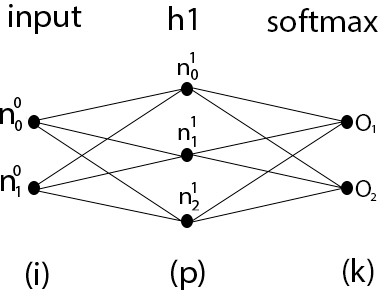
\includegraphics[scale=0.35]{imagenes/nn_1_capa.jpg}  
	\caption{Red Neuronal totalmente conectada con 1 capa oculta}
	\label{fig:nn_1_capa}
\end{figure}

La Figura 3.1 se compone de puntos y líneas, representando neuronas y pesos que las conectan respectivamente. Cada punto es una neurona, y cada línea un peso. \\
La Figura \ref{fig:nn_1_capa} presenta 3 capas (input, h1, output) que corresponden a capa de entrada, capa oculta $h_1$, y capa de salida respectivamente. El superíndice indica la capa a la que pertenece una neurona o peso, mientras que el subíndice indica el número del mismo en su respectiva capa. En el caso de los pesos, se requieren 2 subíndices para identificar a cada uno (pues un peso une 2 neuronas). \\
La capa de entrada se compone de 2 neuronas ($n^{0}_0$ y $n^{0}_1$). \\
La capa oculta $h_1$ tiene 3 neuronas ($n^1_{0}$, $n^1_{1}$, y $n^1_{2}$) \\
El peso $W^{i}_{jk}$ referencia al peso que une las neuronas $n^{i}_j$ y $n^{i+1}_k$.\\
Además, se denotará como $\hat{y}$ a la última neurona de la red, pues contendrá la predicción de la misma.  

\subsubsection{Capa output}

Sea la neurona $n^i_j$, se define como $a^i_j$ el valor de dicha neurona antes de aplicar sobre ella su función de activación asociada, y $z^i_j$ el obtenido tras aplicarla. De forma adicional, se usará $\hat{a}$ y $\hat{z}$ para $\hat{y}$.

Así, la función de pérdida \ref{loss_func} se convierte en:

\begin{gather}
	H(x) = - \frac{1}{N} \sum_{i=1}^{N}  [y_i * log( \hat{z}_i) + (1-y_i)*log(1-\hat{z}_i)]
	\label{loss_func_az}
\end{gather}

Para realizar el descenso del gradiente, se debe empezar calculando la derivada de la función de pérdida respecto a la predicción obtenida. Es decir, la derivada de la fórmula (3.1) respecto de las neuronas en la última capa de la red tras aplicar sus respectivas funciones de activación, que en este caso corresponde a $\hat{z}$. \\
Por simplicidad, podemos dividir esta derivada en 2 partes. \\
Parte izquierda:
\begin{gather}
	f(x) = A*B \\  
	f'(x) = AB' + A'B \\
	\frac{\partial y_i}{\partial \hat{z}_i} = 0 \\
	\frac{\partial log(\hat{z}_i)}{\partial \hat{z}_i} = \frac{1}{\hat{z}_i} \\
	\frac{\partial y_i * log( \hat{z}_i)}{\partial \hat{z}_i} = y_i*\frac{1}{\hat{z}_i} + 0*log(\hat{z}_i) = \frac{y_i}{\hat{z}_i}
\end{gather}

Parte derecha:
\begin{gather}
	\frac{\partial (1-y_i)}{\partial \hat{z}_i} = 0\\
	\frac{\partial log(1-\hat{z}_i)}{\partial \hat{z}_i} = \frac{1}{1-\hat{z}_i} * (-1) \\
	\frac{\partial (1-y_i)*log(1-\hat{z}_i)}{\partial \hat{z}_i} = (1-y_i)*\frac{1}{1-\hat{z}_i}*(-1) + 0* log(1-\hat{z}_i) \\
	\frac{\partial (1-y_i)*log(1-\hat{z}_i)}{\partial \hat{z}_i} = -\frac{1-y_i}{1-\hat{z}_i}
\end{gather}

Finalmente, se obtiene: 
\begin{gather}
	\frac{\partial H(x)}{\partial \hat{z}_i} = - \frac{1}{N} \sum_{i=1}^{N}  [ \frac{y_i}{\hat{z}_i} - \frac{1-y_i}{1-\hat{z}_i} ]
\end{gather}

\subsubsection{Función activación de la capa output}
En la capa output se emplea la función de activación sigmoide. 

\begin{gather}
	sigmoide(x) = \frac{1}{1+e^{-x}} \\
	sigmoide'(x) = \frac{sigmoide(x)}{1-sigmoide(x)}
\end{gather}

De esta forma,

\begin{gather}
	\frac{\partial \hat{z}}{\partial \hat{a}} = \frac{\partial sigmoide(\hat{a})}{\partial \hat{a}} = sigmoide(\hat{a})*(1-sigmoide(\hat{a}))
\end{gather}

Ahora, podemos calcular el gradiente completo hasta la capa output antes de aplicar su función de activación.

\begin{gather}
	grad\_output = \frac{\partial H(x)}{\partial \hat{z}} * \frac{\partial \hat{z}}{\partial \hat{a}} =
	- \frac{1}{N} \sum_{i=1}^{N}  [ \frac{y_i}{\hat{z}_i} - \frac{1-y_i}{1-\hat{z}_i} ] * \frac{\partial \hat{z}}{\partial \hat{a}} \\
	grad\_output = - \frac{1}{N} \sum_{i=1}^{N}  [ \frac{y_i}{\hat{z}_i} - \frac{1-y_i}{1-\hat{z}_i} ] * sigmoide(\hat{a})*(1-sigmoide(\hat{a}))
\end{gather}

\subsubsection{Pesos capas h1-output}

Una vez calculado el gradiente hasta la capa output, se puede calcular el gradiente respecto a cada peso que se encuentra conectado a esta desde la capa anterior. Es decir, para cada $h^1_p\in h_1$, se calcula $\frac{dH(x)}{dW^1_{p\hat{y}}}$. Usando la regla de la cadena, equivale a realizar lo siguiente:

\begin{gather}
	\frac{\partial \hat{y}}{\partial W^1_{p\hat{y}}} = \frac{\partial n^1_p * W^1 _{p\hat{y} }}{\partial W^1_{p\hat{y} }} = n^1_p \\
	\frac{\partial H(x)}{\partial W^1_{p\hat{y} }} = \frac{\partial H(x)}{\partial \hat{y}} * \frac{\partial\hat{z}}{\partial \hat{a}} * \frac{\partial \hat{y}}{\partial W^1_{p\hat{y} }} =  grad\_output * \frac{\partial \hat{y}}{\partial W_{p\hat{y} }} = grad\_output * n^1_p
\end{gather}

\subsubsection{Capa oculta h1}

\begin{gather}
	\frac{\partial \hat{y}}{\partial n^1_p} = \frac{\partial n^1_p * \partial W^1 _{p\hat{y}} }{\partial n^1_p } = \partial W^1_{p\hat{y}} \\
	deriv\_relu(x) = 0\ si\ x <= 0,\ 1\ en\ caso\ contrario \\
	\frac{\partial z^1_p }{\partial a^1_p } = \frac{\partial relu(a^1_p)}{\partial a^1_p } = deriv\_relu(a^1_p) \\
	\frac{\partial H(x) }{\partial n^1_p } = grad\_output* \frac{\partial \hat{y} }{\partial n^1_p } * \frac{\partial z^1_p }{\partial a^1_p } = grad\_output * W^1_{p\hat{y} } * deriv\_relu(a^1_p ) \\
	\frac{\partial H(x) }{\partial n^1_p } = gradient\_n^1_p
\end{gather}

\subsubsection{Pesos capas input-h1}

\begin{gather}
	\frac{\partial n^1_p }{\partial W^0_{ip} } = \frac{\partial n^0_i * W^0_{ip} }{\partial W^0_{ip} } = n^0_i \\
	\frac{\partial H(x) }{\partial W^0_{ip} } = gradient\_n^1_p * \frac{\partial n^1_p }{\partial W^0_{ip} } = gradient\_n^1_p * n^0_i 
\end{gather}


\subsubsection{Capa input}

\begin{gather}
	\frac{\partial n^1_p }{\partial n^0_i } = \frac{\partial n^0_i * W^0_{ip} }{\partial n^0_i } = W^0_{ip} \\
	\frac{\partial z^0_i }{\partial a^0_i } = 1
\end{gather}

Ahora se realiza una sumatoria con todos los 'caminos posibles' hacia la misma neurona
\begin{gather}
	\frac{\partial H(x) }{\partial n^0_i } = \sum_{p=0}^{h_1.size()} gradient\_n^1_p * \frac{\partial n^1_p }{\partial n^0_i } * \frac{\partial z^0_i }{\partial a^0_i }  \\
	\frac{\partial H(x) }{\partial n^0_i } = \sum_{p=0}^{h_1.size()}  gradient\_n^1_p * W^0_{ip}
\end{gather}

